\setcounter{chapter}{0}
\chapter{Introduction}
\section{Problématique}
\section{Définitions}
\subsection{Agent intelligent}
Un agent est un logiciel qui agit de façon autonome. C'est un programme qui accomplit des tâches à la manière d'un automate et en fonction de ce que lui a demandé son auteur, en revanche un \textbf{agent intelligent} est une entité autonome capable de percevoir son environnement grâce à des capteurs et aussi d'agir sur celui-ci via des effecteurs afin de réaliser des buts1. Un agent intelligent peut également apprendre ou utiliser des connaissances pour pouvoir réaliser ses objectifs.
\begin{figure}[H]
	\centering
	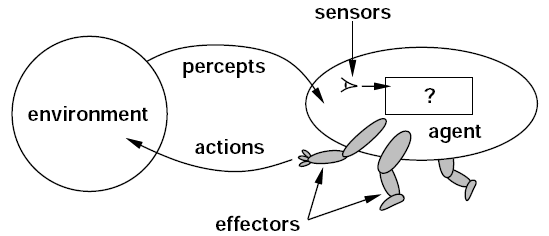
\includegraphics[width=0.5\textwidth]{imgs/intelligentAgent.png}
	\caption{Agent intelligent interagissant avec le monde extérieur }
\end{figure}
\newpage
\subsection{Système multi-agents}
un système multi-agents (SMA) est un système composé d'un ensemble d'agents (un processus, un robot, un être humain, etc.), situés dans un certain environnement et interagissant selon certaines relations. Un agent est une entité caractérisée par le fait qu'elle est, au moins partiellement, autonome.
\begin{figure}[H]
	\centering
	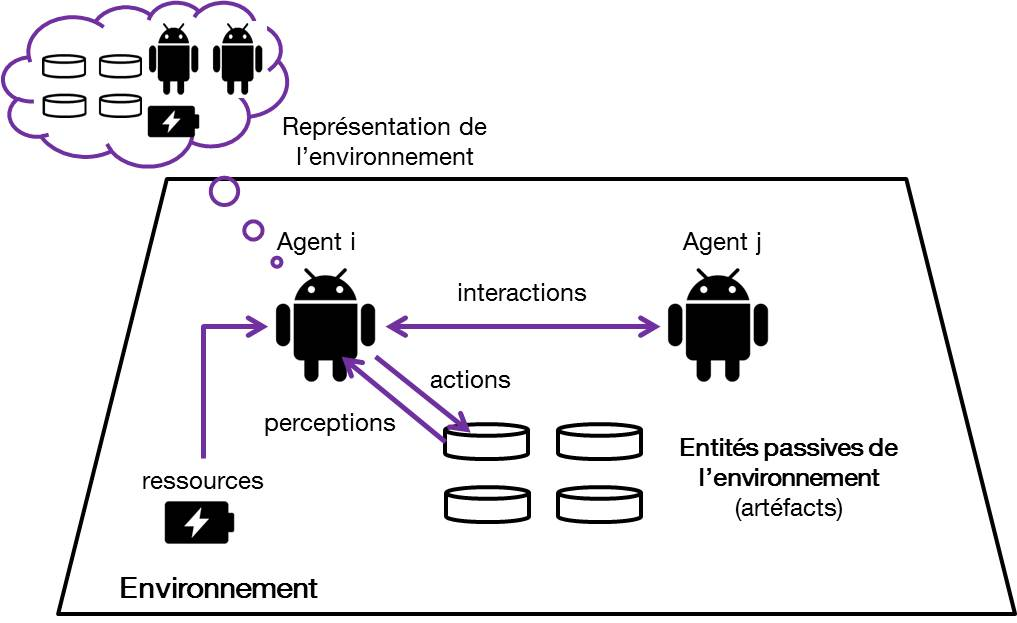
\includegraphics[width=0.5\textwidth]{imgs/SMA.jpg}
	\caption{Système multi-agents en coopération}
\end{figure}